\chapter{Launch and Astrodynamic Characteristics}
\label{frLaAC}
This chapter explains the characteristics of the launch and space segments of the mission. Section \ref{frLS} describes the three main characteristics of bringing the swarm into the orbit: launch vehicle, launch location and orbit insertion. Section \ref{frSS} discusses all the aspects of the constellation and its configuration, and delves into estimations of $\Delta$V and needed propellant. Finally, section \ref{frSEaS} deals with the hazardous space environment and ways of protecting the satellites against it. 

\section{Launch Segment}
\label{frLS}

The launch segment of the mission includes the selection of the launch vehicle, the launch location and the procedure of inserting the satellites into their respective orbits. The following subsections discuss all of these aspects. 

\subsection{Launch Vehicle}
\label{frLSLV}

The costs of launch vary greatly between different vehicles. Table \ref{table:vehicleCosts} on page \pageref{table:vehicleCosts} lists approximate total launch costs of respective platforms. The prices are given in Fiscal Year 2000 dollars for consistency.
\begin{table}[h]
\begin{centering}
\begin{tabular}{llr}
\toprule
Platform & Operator & Price (FY00\$m) \\
\hline \hline
Ariane V  & ESA & 97.96 \\
Soyuz   & Starsem or Arianespace&  8.16 - 22.1 \\
Vega   & European and Italian SA  & 15.1 \\
Falcon 1E  & SPACEX  & 8.89 \\
PSLV & ISRO & 13.88 - 16.33 \\
Rokot & Eurokot & 9.8 - 11.4 \\
\bottomrule
\end{tabular}
\caption{Estimated price comparison of different launch vehicles. \emph{Source: various.}}
\label{table:vehicleCosts}
\end{centering}
\end{table}

Based on the information  in the above table it is possible to single out a few platforms which will be affordable for the purpose of this feasibility study. The values represent the total launch segment costs. The Ariane V launcher is the most expensive option by far and would push the budget quite heavily, with an estimated cost of launch almost half of the total budget. However the payload capabilities of the Ariane V launcher far outweigh that of all other platforms, thus making it possible for a combined launch with other satellites, leading to shared costs. This however could jeopardize the mission in the sense that it becomes secondary priority. If that happens, the constellation would have have have higher requirements for orbit acquisition: an extra booster stage or higher onboard fuel capacity for the altitude and/or plane shift, which is not feasible. The Ariane V is therefore an unsuitable platform for this project. 

The rest of the launchers can be analyzed with respect to reliability. All of the launch vehicles have been tested, with the exception of the Vega system, which is yet to make its maiden flight. The Vega is therefore not suitable for the analysis at this time. It is for this reason that the project will no longer consider this system at all.  However, better data should be available in the near future which should allow for the Vega platform to be reevaluated.

The same goes for the Falcon - 1e system. The launcher is still under development. Furthermore, the predecessor of the 1e system is the Falcon - 1, which out of total of five launches only had two successful, fails to make a favorable impression. 

Table \ref{table:LVreliability} on page \pageref{table:LVreliability} shows some reliability statistics for the remaining 3 vehicles.

\begin{table}[h]
\begin{centering}
\begin{tabular}{lcccp{5cm}}
\toprule
Platform & Total No. of Launches & Total Failures & Reliability & No. of Successful Launches Since Last Failure  \\
\hline \hline
Soyuz   & 1754  &  88 & 95\% & 57 \\
PSLV & 16 & 1 & 94\% & 15 \\
Rokot & 17& 2 & 88\% & 6 \\
\bottomrule
\end{tabular}
\caption{Reliability figures for several launch vehicles. \emph{Source: various.} }
\label{table:LVreliability}
\end{centering}
\end{table}

The Soyuz launch vehicle presents itself as the most reliable platform, with a track record that far surpassed all other options. This launch vehicle will be the one considered for this project. In the next section, its payload capabilities are discussed.

\subsubsection{Soyuz LV Payload Capability Analysis}
\label{frLVPCA}

There is a large selection of Soyuz vehicles available for consideration. For the purpose of this project, the newest modification - Soyuz-ST will be used. This vehicle is part of the Soyuz-2 family, which are technologically superior to the older Soyuz-U and U2 launchers. An illustration and technical parameters of the Soyuz-ST can be found in Appendix \ref{appa} on page \pageref{appa} \cite{soyuzman}.

An estimation of mass performance for the launch vehicle can be seen in figure \ref{fig:massperformance} on page \pageref{fig:massperformance}.

\begin{figure}[ht]
\centering
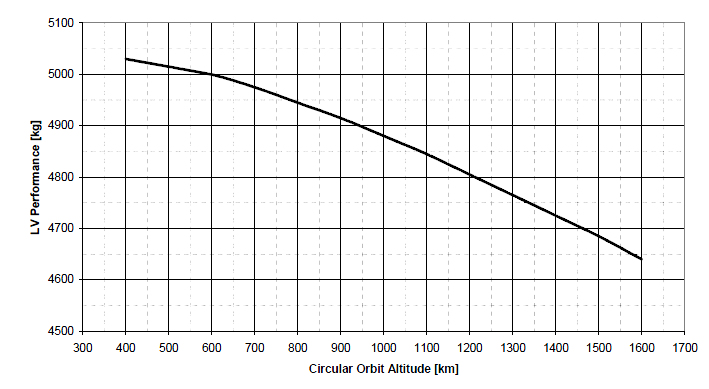
\includegraphics[width=1.0\textwidth, angle=0]{chapters/img/lvmass.png}
\caption{Mass performance of the Soyuz-ST for circular Orbits.\emph{ Source: \cite{soyuzman}.}}
\label{fig:massperformance}
\end{figure}

The payload mass data provided in \cite{soyuzman} is estimated, yet is good enough to have a reasonable idea about the maximum mass. The Soyuz-ST is able to launch roughly a maximum of 5000 kg into a 500km orbit. This is well above the design mass of the formation thus will allow for further considerations of joint launches (as long as the swarm mission is considered to be the primary payload) and thus spread launch costs. 

The available volume in the Soyuz-ST Fairing can be seen in figure \ref{fig:soyuzvol} on page \pageref{fig:soyuzvol}.

\begin{figure}[!h]
\centering
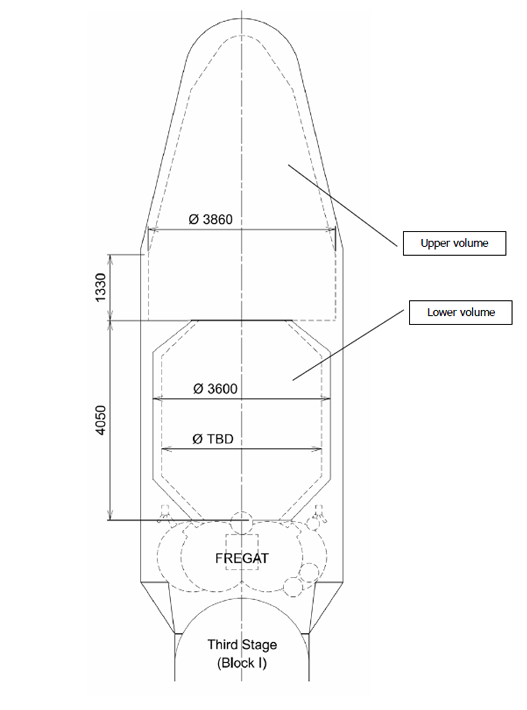
\includegraphics[scale = 0.5, angle=0]{chapters/img/soyuzvol.png}
\caption{Fairing volume of the Soyuz-ST launch vehicle. Here shown in dual launch carrying configuration.\emph{ Source: \cite{soyuzman}.}}
\label{fig:soyuzvol}
\end{figure} 

The dimensions of the fairing are visibly too large and there is no possibility of using a different one, however that leaves a lot of possibilities for different designs of release adapters to adapt to the unique sequence of separation upon orbit injection. Again, the possibility of taking other small satellites along on the same launch arises. The dual launch configuration shown in the previous figure is the one being considered for the launch.

The choice of the Soyuz brings forth one more advantage: the use of a unique orbit insertion booster, the Fregat. This final stage will allow for minimization of fuel on the satellite as all orbit insertion maneuvers can be done using the Fregat. The Fregat stage has been designed to handle 20 individual burns.

\subsubsection{Vibrational Analysis}
\label{frLVCA}

HERE ADD VIBRATION ANALYSIS  

\subsection{Launch Site}
\label{frLSLS}

The selection of the launch site relies on several factors:

\begin{itemize}
	\item Availability of attainable inclinations from launch.
	\item Compatibility with the launch vehicle.
	\item Accessibility and cost.
	\item Security and political reasons. 
\end{itemize}

The first factor is crucial. It is paramount that the satellites are injected into their final inclinations at launch and do not have to perform any inclination change maneuvers, which require a substantial $\Delta$V. With this in mind choosing a launch site closer to the equator is necessary. Launch sites at higher latitudes would need to sacrifice velocity and thus payload mass because of their location. Table \ref{table:launchtable} on page \pageref{table:launchtable} shows a number of possible launch sites and their locations \cite{larson}. The list contains only the sites compatible with the Soyuz-ST launch vehicle. Furthermore, in figure \ref{fig:launchsites} on page \pageref{fig:launchsites}, the same sites are indicated with their respective authorized inclination ranges.

\begin{table}[!h]
\begin{centering}
\begin{tabular}{llp{2cm}p{2cm}}
\toprule
Launch Site & Operator & Latitude (deg min) & Longitude (deg min) \\
\hline \hline
Baikonur LC-31/6  & Russia (Starsem) & 45 54 N & 63 18 E \\
Plesetsk LC-43  & Russia (Starsem)   &  62 48 N & 40 24 E \\
Guiana Space Centre  ELS  & CNES/Arianespace  & 5 18 N & 52 50 W \\
\bottomrule
\end{tabular}
\caption{Available launch sites for the Soyuz-ST.   \emph{Source: \cite{larson}.}}
\label{table:launchtable}
\end{centering}
\end{table}  

\begin{figure}[!h]
\centering
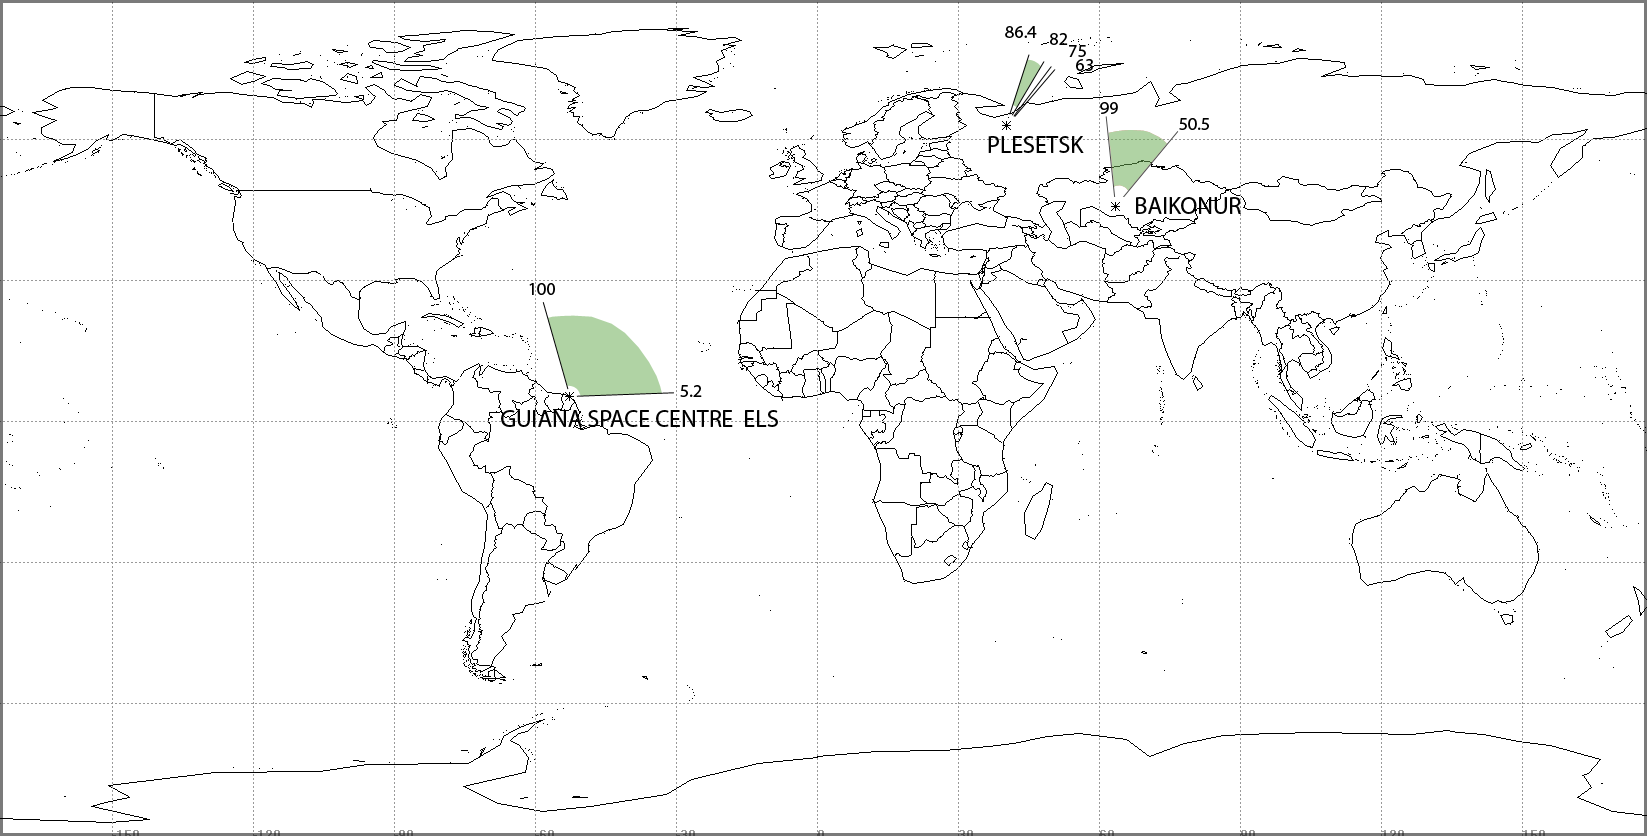
\includegraphics[width=1.0\textwidth, angle=0]{chapters/img/launchsites.png}
\caption{Launch site locations and allowable inclinations for the Soyuz-ST. \emph{Sources: \cite{constDesign} and \cite{rockotman}.} }
\label{fig:launchsites}
\end{figure}

Even though all the above sites allow inclinations of 85 degrees, it is still preferable to select a site closer to the equator in order to utilize the full effect of Earth's rotation and lower the launch costs. With this in mind, the Guiana Space Centre is selected to be the preferable location for launch.

The \ac{ELS} in Kourou, Guiana is currently being finalized and should accommodate its first Soyuz launch in 2010 \cite{arianesoyuz}.

A typical launch profile of the Soyuz launch vehicle from Kourou is shown in figure \ref{fig:launch} on page \pageref{fig:launch}. The first three stages of the vehicle are used propel the payload and the Frigate booster to a circular orbit at around 200 km. After separation (stage 6 on the figure), the Fregat initiates the first orbit injection burn to bring the satellites to the appropriate orbits.

\begin{figure}[!h]
\centering
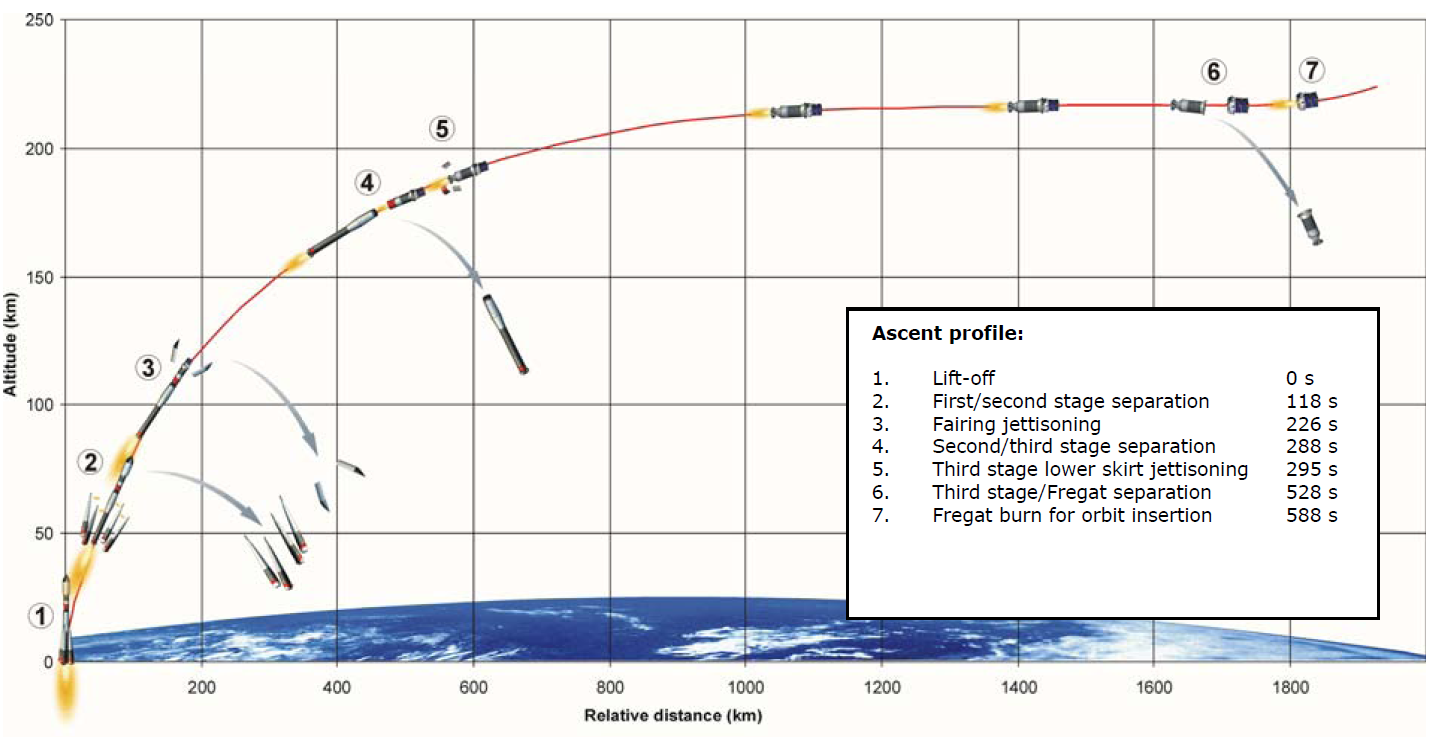
\includegraphics[width=1.0\textwidth, angle=0]{chapters/img/launchprofile.png}
\caption{Launch profile of the Soyuz LV from Kourou. \emph{Sources: \cite{soyuzman}.} }
\label{fig:launch}
\end{figure}

With this information it is possible to further calculate some important launch parameters:

\begin{itemize}
	\item The inertial velocity of the launch site is given by:
	
	\begin{equation} 
 		V_L = (464.5) cos L 
	\end{equation}
	
	where $L$ is the site latitude. For the case of Kourou the inertial velocity is 462.51 m/s.
	\item The launch azimuth in inertial frame of reference is given by:
	
	\begin{equation} 
 		A_{Z_I} = arcsin(\frac{cos i}{cos L})
	\end{equation}
	
	and is equal to 5.022 degrees for this launch.
	\item The launch azimuth corrected for the Earth's rotation, is given by:
	
	\begin{equation} 
 		A_Z = arctan(\frac{V_0sinA_{Z_I}-V_{eq}cosL}{V_0cosA_{Z_I}})
	\end{equation}
	
	where $V_0$ is the orbital velocity reached by the launcher before separation and the first burn of Fregat upper stage (see above, around 7.784 km/s), $V_{eq}$ is the velocity of the Earth's rotation at the equator - 464.5 m/s. Thus the corrected launch azimuth becomes 1.61 degrees. 
	
	\item The required launch velocity is calculated to be 7.76 km/s which means that due to Earth's rotation 26.8 m/s are saved.
\end{itemize}

Furthermore the region is politically stable and the launch site is under the protection from the French government and other security forces. All safety procedures are kept to the highest of standards and the spaceport is easily accessible by air or sea \cite{soyuzman}.

\subsection{Orbit Insertion}
\label{frLSOI}

The orbit insertion is separated into two distinct stages: primary orbits and secondary orbits. The primary orbits are located at an altitude of 500 km and contain the emitter and four initial receivers. The secondary orbits are located at a slightly different altitude of 550 (CHECK ALTITUDE!!!!) km and contain the auxiliary receivers intended for replenishment.

The configuration of the primary orbits is discussed in section \ref{frSSSC} and an image of the formation can be seen in figure \ref{fig:confmax} on page \pageref{fig:confmax}. The release sequence and the important parameters are as follows (for satellite and orbit numbers please refer to figure \ref{fig:confmax}):

\begin{enumerate}
	\item The Fregat is injected in Orbit 1.
	\item The ascending intersection of Orbit 1 and Orbit 2 is reached at a latitude of 85$^{\circ}$ and a longitude offset (from the ascending node of Orbit 1) of 88.91$^{\circ}$. At this point the Fregat should be orientated in the direction of Orbit 2 and separate Rec 2. The separation $\Delta$V that the adapter should produce is calculated using:
	
	\begin{equation} 
 		\Delta V = 2 V_i sin \frac{\alpha}{2}
	\end{equation}
	
	where $V_i$ is the orbital velocity (7.612 km/s) and $\alpha$ is the relative inclination (2.17$^{\circ}$, see section \ref{frSSSC}) \cite{spacedesign}. The $\Delta$V is calculated to be 289.63 m/s.
	
	\item As the Fregat crosses the descending node and approaches the second plane intersection of the orbit, it does not need to change orientation (Orbit 3 intersects in the same direction on the descent phase as Orbit 2 does on the ascent phase). At the intersection Rec 1 is separated with a $\Delta$V of 289.63 m/s.
	\item After this the Fregat again aligns with the velocity vector of Orbit 1.
	\item The Frigate should inject itself into a drift orbit with a negative drift rate of no less then 9.19 deg/orbit and re-injected back to Orbit 1 after traveling $90+\Delta \phi /2 = 90.09505$ degrees. This will bring the launcher 2.3 degrees behind the final emitter position, or 0.12 degrees behind Rec 4.
	\item At this point the remaining three satellites: Rec 3, Base and Rec 4 should be put into drift orbits by the attachment mechanism in order to acquire the 2.18 degree orbital separation. The exact order and timing can be designed and adjusted accordingly.
\end{enumerate}

After this, the satellites can be considered to be in their orbits. The Fregat can start the burn to insert into the secondary orbits. The formation in the secondary orbit is the same as in the primary orbits minus the emitter, thus similar maneuvers have to be performed.

\subsection{Launch Date}
\label{frLSLD}

The launch date is dominated by development times and lifetime considerations. The satellite orbit decay is and thus lifetime is a function of atmospheric density. The density is, in turn, a function of the solar activity. The number of sun spots on the surface of the sun rises and falls every eleven years. The measurements are commonly represented in 10.7cm radio flux intensities. Figure \ref{fig:f10.7} on page \pageref{fig:f10.7} presents a projection for the next 10 years.

\begin{figure}[!h]
\centering
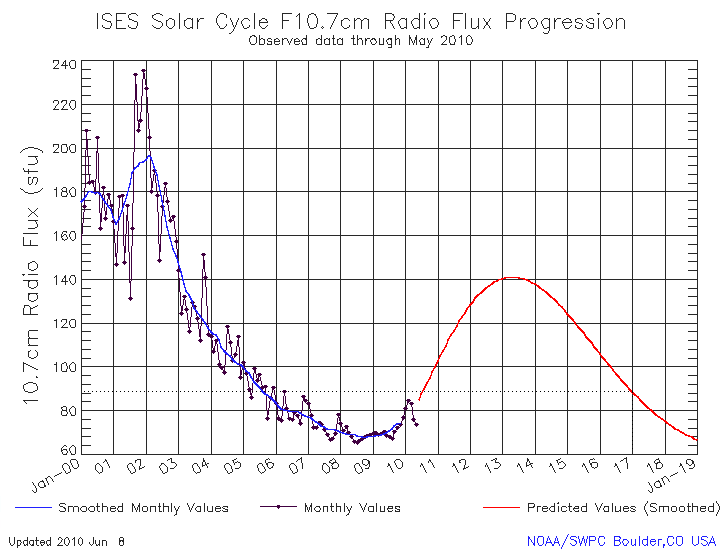
\includegraphics[width=1.0\textwidth, angle=0]{chapters/img/solarCycle.png}
\caption{Solar activity projection up to 2019. \emph{Source: NOAA/Space Weather Prediction Center.} }
\label{fig:f10.7}
\end{figure}

In order to provide the longest possible lifetime for the mission it is essential that the launch is timed in such a way that the satellites are in orbit most of the time during solar minimum. For this reason a launch on March 1st 2017 is planned. This also gives enough time for development and production. For further information on the timeline, please refer to section \ref{frPMGC}.

\section{Space Segment}
\label{frSS}

This section covers the astrodynamical characteristics of the mission. Emitter orbit is covered first, then in section \ref{frSSRO}, all receiver orbits are examined. The formation and its properties are discussed in section \ref{frSSSC}. Collision avoidance is described in section \ref{frSSCA} and, finally, section \ref{frSEaS} covers the orbital environment and whether the mission is going to be heavily affected by it. 

\subsection{Emitter Orbit}
\label{frSSEOD}

The emitter satellite is injected into a circular orbit at an altitude of 500 km. The eccentricity is frozen at 0. Inclination is chosen to be 85 degrees. 

\subsection{Receiver Orbits}
\label{frSSRO}

b lss

\subsection{Swarm Configuration}
\label{frSSSC}

\begin{figure}[!ht]
\centering
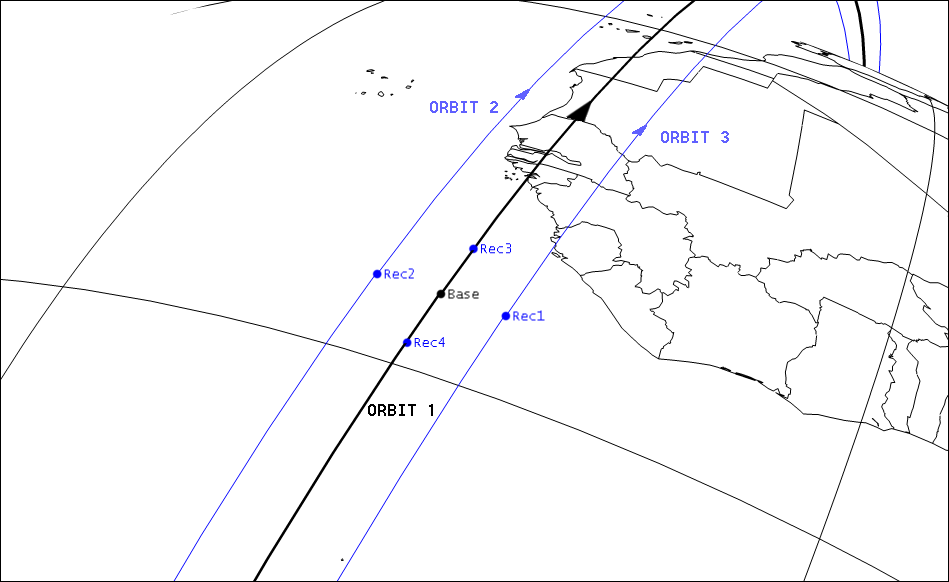
\includegraphics[width=0.8\textwidth, angle=0]{chapters/img/primaryconfmax.png}
\caption{Swarm configuration as seen when the emitter (labeled here as Base) crosses its ascending node. Orbit numbers represent the different orbital planes.}
\label{fig:confmax}
\end{figure}

\begin{figure}[!h]
\centering
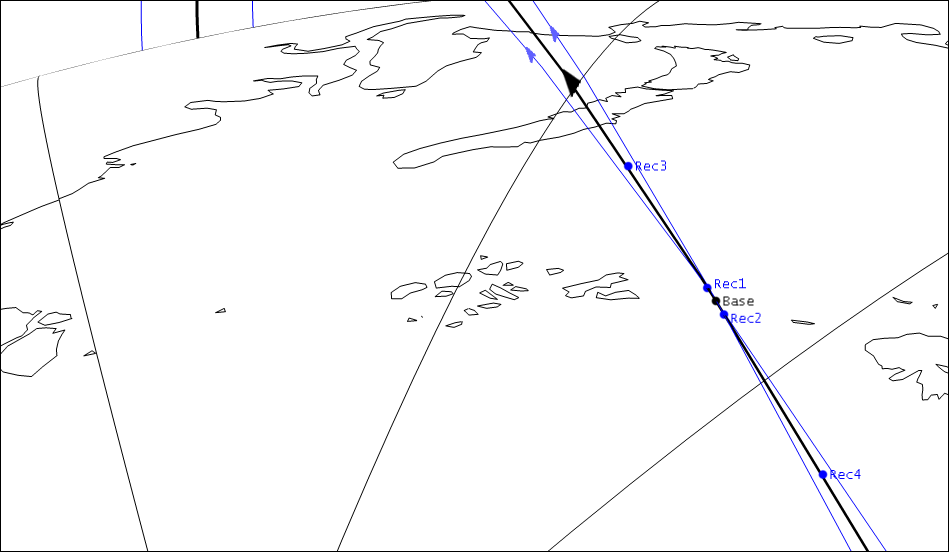
\includegraphics[width=0.8\textwidth, angle=0]{chapters/img/primaryconfmin.png}
\caption{Swarm configuration as seen when the orbit planes intersect. In this figure the intersection in ascent is pictured.}
\label{fig:confmin}
\end{figure}

\subsection{Collision Avoidance}
\label{frSSCA}

bla

\section{Space Environment and Shielding}
\label{frSEaS}

Bla